\documentclass[12pt,a4paper]{report}
\usepackage[utf8]{inputenc}
\usepackage[russian]{babel}
\usepackage[OT1]{fontenc}
\usepackage{amsmath}
\usepackage{amsfonts}
\usepackage{amssymb}
\usepackage{graphicx}
\usepackage{cmap}					% поиск в PDF
\usepackage{mathtext} 				% русские буквы в формулах
%\usepackage{tikz-uml}               % uml диаграммы



% Генератор текста
\usepackage{blindtext}

%------------------------------------------------------------------------------

% Подсветка синтаксиса
\usepackage{color}
\usepackage{xcolor}
\usepackage{listings}
 
 % Цвета для кода
\definecolor{string}{HTML}{B40000} % цвет строк в коде
\definecolor{comment}{HTML}{008000} % цвет комментариев в коде
\definecolor{keyword}{HTML}{1A00FF} % цвет ключевых слов в коде
\definecolor{morecomment}{HTML}{8000FF} % цвет include и других элементов в коде
\definecolor{captiontext}{HTML}{FFFFFF} % цвет текста заголовка в коде
\definecolor{captionbk}{HTML}{999999} % цвет фона заголовка в коде
\definecolor{bk}{HTML}{FFFFFF} % цвет фона в коде
\definecolor{frame}{HTML}{999999} % цвет рамки в коде
\definecolor{brackets}{HTML}{B40000} % цвет скобок в коде
 
 % Настройки отображения кода
\lstset{
language=C, % Язык кода по умолчанию
morekeywords={*,...}, % если хотите добавить ключевые слова, то добавляйте
 % Цвета
keywordstyle=\color{keyword}\ttfamily\bfseries,
stringstyle=\color{string}\ttfamily,
commentstyle=\color{comment}\ttfamily\itshape,
morecomment=[l][\color{morecomment}]{\#}, 
 % Настройки отображения     
breaklines=true, % Перенос длинных строк
basicstyle=\ttfamily\footnotesize, % Шрифт для отображения кода
backgroundcolor=\color{bk}, % Цвет фона кода
%frame=lrb,xleftmargin=\fboxsep,xrightmargin=-\fboxsep, % Рамка, подогнанная к заголовку
frame=tblr
rulecolor=\color{frame}, % Цвет рамки
tabsize=3, % Размер табуляции в пробелах
showstringspaces=false,
 % Настройка отображения номеров строк. Если не нужно, то удалите весь блок
numbers=left, % Слева отображаются номера строк
stepnumber=1, % Каждую строку нумеровать
numbersep=5pt, % Отступ от кода 
numberstyle=\small\color{black}, % Стиль написания номеров строк
 % Для отображения русского языка
extendedchars=true,
literate={Ö}{{\"O}}1
  {Ä}{{\"A}}1
  {Ü}{{\"U}}1
  {ß}{{\ss}}1
  {ü}{{\"u}}1
  {ä}{{\"a}}1
  {ö}{{\"o}}1
  {~}{{\textasciitilde}}1
  {а}{{\selectfont\char224}}1
  {б}{{\selectfont\char225}}1
  {в}{{\selectfont\char226}}1
  {г}{{\selectfont\char227}}1
  {д}{{\selectfont\char228}}1
  {е}{{\selectfont\char229}}1
  {ё}{{\"e}}1
  {ж}{{\selectfont\char230}}1
  {з}{{\selectfont\char231}}1
  {и}{{\selectfont\char232}}1
  {й}{{\selectfont\char233}}1
  {к}{{\selectfont\char234}}1
  {л}{{\selectfont\char235}}1
  {м}{{\selectfont\char236}}1
  {н}{{\selectfont\char237}}1
  {о}{{\selectfont\char238}}1
  {п}{{\selectfont\char239}}1
  {р}{{\selectfont\char240}}1
  {с}{{\selectfont\char241}}1
  {т}{{\selectfont\char242}}1
  {у}{{\selectfont\char243}}1
  {ф}{{\selectfont\char244}}1
  {х}{{\selectfont\char245}}1
  {ц}{{\selectfont\char246}}1
  {ч}{{\selectfont\char247}}1
  {ш}{{\selectfont\char248}}1
  {щ}{{\selectfont\char249}}1
  {ъ}{{\selectfont\char250}}1
  {ы}{{\selectfont\char251}}1
  {ь}{{\selectfont\char252}}1
  {э}{{\selectfont\char253}}1
  {ю}{{\selectfont\char254}}1
  {я}{{\selectfont\char255}}1
  {А}{{\selectfont\char192}}1
  {Б}{{\selectfont\char193}}1
  {В}{{\selectfont\char194}}1
  {Г}{{\selectfont\char195}}1
  {Д}{{\selectfont\char196}}1
  {Е}{{\selectfont\char197}}1
  {Ё}{{\"E}}1
  {Ж}{{\selectfont\char198}}1
  {З}{{\selectfont\char199}}1
  {И}{{\selectfont\char200}}1
  {Й}{{\selectfont\char201}}1
  {К}{{\selectfont\char202}}1
  {Л}{{\selectfont\char203}}1
  {М}{{\selectfont\char204}}1
  {Н}{{\selectfont\char205}}1
  {О}{{\selectfont\char206}}1
  {П}{{\selectfont\char207}}1
  {Р}{{\selectfont\char208}}1
  {С}{{\selectfont\char209}}1
  {Т}{{\selectfont\char210}}1
  {У}{{\selectfont\char211}}1
  {Ф}{{\selectfont\char212}}1
  {Х}{{\selectfont\char213}}1
  {Ц}{{\selectfont\char214}}1
  {Ч}{{\selectfont\char215}}1
  {Ш}{{\selectfont\char216}}1
  {Щ}{{\selectfont\char217}}1
  {Ъ}{{\selectfont\char218}}1
  {Ы}{{\selectfont\char219}}1
  {Ь}{{\selectfont\char220}}1
  {Э}{{\selectfont\char221}}1
  {Ю}{{\selectfont\char222}}1
  {Я}{{\selectfont\char223}}1
  {і}{{\selectfont\char105}}1
  {ї}{{\selectfont\char168}}1
  {є}{{\selectfont\char185}}1
  {ґ}{{\selectfont\char160}}1
  {І}{{\selectfont\char73}}1
  {Ї}{{\selectfont\char136}}1
  {Є}{{\selectfont\char153}}1
  {Ґ}{{\selectfont\char128}}1
  {\{}{{{\color{brackets}\{}}}1 % Цвет скобок {
  {\}}{{{\color{brackets}\}}}}1 % Цвет скобок }
}
 
 % Для настройки заголовка кода
\usepackage{caption}
\DeclareCaptionFont{white}{\color{сaptiontext}}
\DeclareCaptionFormat{listing}{\parbox{\linewidth}{\colorbox{сaptionbk}{\parbox{\linewidth}{#1#2#3}}\vskip-4pt}}
\captionsetup[lstlisting]{format=listing,labelfont=white,textfont=white}
\renewcommand{\lstlistingname}{Код} % Переименование Listings в нужное именование структуры


%------------------------------------------------------------------------------

\author{М.В.Булгакова}
\title{Лабораторная работа по программированию \\ "Электронный школьный дневник"}
\begin{document}
\maketitle
\chapter{Электронный школьный дневник}
\section{Введение}
Школьный дневник, — основной документ школьника на время обучения. Дневник выполняет функции журнала регистрации оценок, полученных на уроках, замечаниях по поведению, средства общения учителей и родителей, а также показатель успеваемости ученика. В современном мире уже давно существует практика электронного школьного дневника. Данная лабораторная демонстрирует еще один вид электронного дневника школьника. 
\section{Задание}

Создать проект "Электронный школьный дневник". Электронный школьный дневник - программа, позволяющая выставлять оценки за модуль, вычислять полугодовую и годовую оценки учащихся, просчитывать процент успеваемости класса, также реализовывающая поиск отличников, хорошистов и троечников.
\section{Концепция}

Программа должна предоставлять ученику/родителю возможность просмотра табеля данного ученика, процент его успеваемости. Учитель в отличие от ученика/родителя имеет права на изменение оценок, так же может запросить список и количество отличников/хорошистов/троечников и процент успеваемости всего класса, так и отдельных учеников.

\section{Минимально работоспособный продукт(MVP)}
Программа, которая позволяет ученику/родителю возможность просмотра оценок данного ученика за год, и которая предоставляет учителю права на запрос список/количество отличников/хорошистов/троечников и процент успеваемости всего класса, так и отдельных учеников.
\section{Диаграмма прецендентов использования}
\begin{figure}[h]
\center{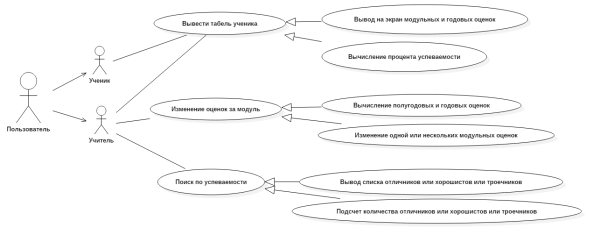
\includegraphics[scale=0.5]{diagrams/UseCaseDiagram1.png}}
\caption{}
\label{fig:image}
\end{figure}
На рис 1.1 изображена диаграмма прецендентов использования. Пользователь авторизируется вначале. И в зависимости от своего статуса ему предлагаются различные функции

\section{Вывод}
В данном разделе определены концепция готового приложения и MVP. Кроме того, в разделе представлена диаграмма прецендентов использования 

\chapter{Проектирование}
\section{Выделенные подпроекты}
В процессе проектирования были выделены 4 подпроекта:
\begin{enumerate}
\item Core - Библиотека приложения
\item APP - Консольное приложение
\item Графическое приложение(нериализовано)
\item Тесты(нериалезованы)
\end{enumerate}
\section{Описание элементов библиотеки}
Интерфейс библиотеки содержит следующие методы:

\begin{verbatim}void marks(student *);\end{verbatim} - Метод, позволяющий найти среднюю оценку ученика, его успеваемость, качество выполнения работы
\begin{verbatim}void find_excelllent_pupil(student *);\end{verbatim}  - Метод, реализующий поиск отличников
\begin{verbatim}void find_good_pupil(student *);\end{verbatim} - Метод, реализующий поиск хорошистов
\begin{verbatim}void find_lagging_pupil(student *);\end{verbatim} - Метод, реализующий поиск отстоющих учеников
\begin{verbatim}void performance_calculation(student *);\end{verbatim} - Метод, вычисляющий успеваемость всего класса, качество выполнения работы, среднюю оценку
\section{Диаграмма компонентов}
\begin{figure}[h]
\center{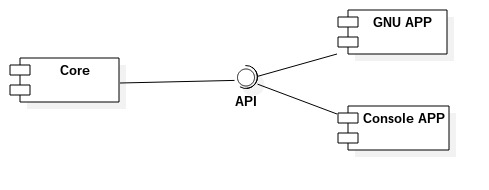
\includegraphics[scale=0.5]{diagrams/ComponentDiagram1.jpg}}
\caption{}
\label{fig:image}
\end{figure}
На рис 2.1 представлена диаграмма компонентов, показывающая зависимости между основными компонентами приложения


\section{Вывод}
В данном разделе рассмотрен процесс проектирования приложения. Описаны выделенные подпроекты и методы интерфейса библиотеки, некоторые подпроекты не были реализованы из-за неправильного планирования разработки всего проекта. 
\chapter{Реализация приложения}
\section{Среда разработки}
Операционная система: Debian(32-bit)
Для создания проекта использовались Qt Creator 3.5.0 (opensource) и GCC.

\section{Выделенные классы}
В библиотеки выделено 3 класса:
\begin{enumerate}
\item Pupil - содержит основную информацию об ученике. Позволяет найти качество, успеваемость и среднюю оценку ученика.
\item Teacher - содержит основную информацию об учителе. Позволяет найти количество отличников, хорошистов, отстающих. Вычисляет качество, успеваемость, среднюю оценку всего класса.
\item CoreAPI - интерфейс ядра.
\end{enumerate}

В подпроекте АРР выделено 3 класса, обеспечивающих взаимодействия пользователя с ядром через консоль:
\begin{enumerate}
\item АPupil
\item АTeacher 
\item menu
\end{enumerate} 


\section{Примеры работы консольного приложения}
Для демонстрации работы консольного приложения ниже приведены снимки экрана работающего приложения.
\begin{enumerate}
\item
\begin{figure}[h!]
\center{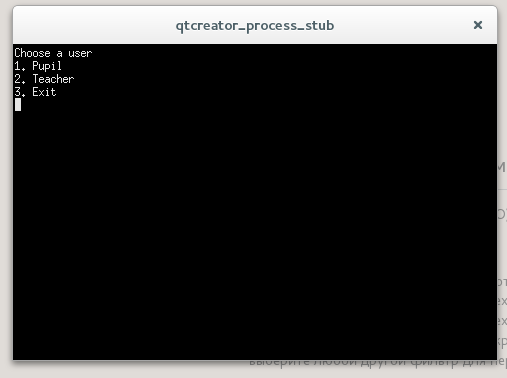
\includegraphics[scale=0.5]{diagrams/1.png}}
\caption{рис1}
\label{fig:image}
\end{figure}
На рис.1 представлено главное меню приложения
\item
\begin{figure}[h!]
\center{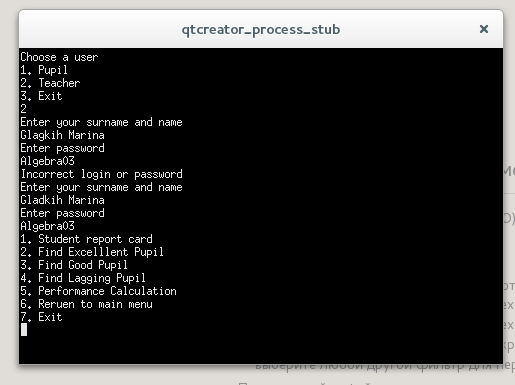
\includegraphics[scale=0.5]{diagrams/2.png}}
\caption{рис2}
\label{fig:image}
\end{figure}
На рис.2 показан пример аутентификации учителя и его меню \newpage
\item
\begin{figure}[h!]
\center{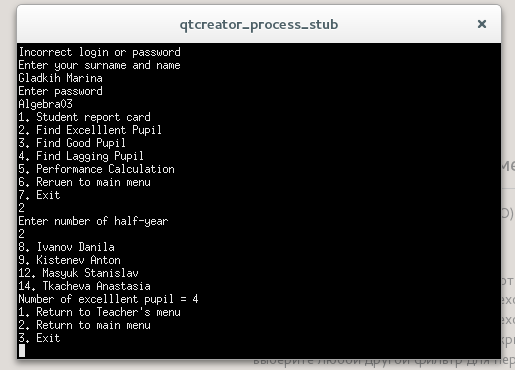
\includegraphics[scale=0.5]{diagrams/3.png}}
\caption{рис3}
\label{fig:image}
\end{figure}
На рис.3 представлен пример поиска отличников во втором полугодии
\item
\begin{figure}[h!]
\center{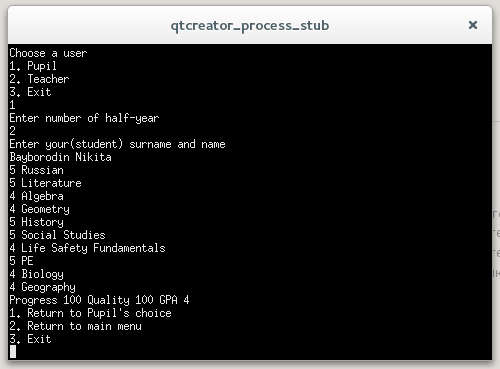
\includegraphics[scale=0.5]{diagrams/4.png}}
\caption{рис4}
\label{fig:image}
\end{figure}
На рис.4 представлен вход от имени ученика
\end{enumerate} 

\section{Выводы}

В данном разделе были описаны классы, выделенные при разработки приложения. Были сделаны снимки экрана, демонстрирующие работу консольного приложения

\chapter{Обеспечение качества}
\section{Просмотр кода и демонстрации}
В ходе разработки приложения были осуществлены 3 демонстрации, в ходе которых были выявлены ошибки работы программы и мелкие недочеты, были высказаны пожелания по функциональности. Все замечания были исправлены, а пожелания реализованы.
Примером пожелания была кнопка выхода и возвращения в меню.
\section{Тестирование}
В ходе работы производилось ручное тестирование программы. Функциональные тесты, покрывающие часть ядра, были удалены, так как после изменение не компилировались, а на поиск ошибок времени не осталось.

\section{Вывод}
В данном разделе описаны демонстрации. Просмотр кода не осуществлялся, но автор понял, что пренебрегать им нелья, так как он помогает выявить ошибки, незамеченные самим автором.

\chapter{Выводы}
Во время разработки приложения автор узнал возможности с++ и лучше усвоил принципы объектно-ориентированного программирования.
Данная программа еще не закончена. Разработка графического интерфейса и покрытие тестами будет осущетсвляться до сентября текущего года.

\chapter*{Листинги}
\lstinputlisting[]
{../sources/RecordBook/APP/apupil.h}

\lstinputlisting[]
{../sources//RecordBook/APP/apupil.cpp}

\lstinputlisting[]
{../sources//RecordBook/APP/ateacher.h}

\lstinputlisting[]
{../sources/RecordBook/APP/ateacher.cpp}

\lstinputlisting[]
{../sources//RecordBook/APP/main.cpp}
\lstinputlisting[]
{../sources//RecordBook/APP/menu.h}
\lstinputlisting[]
{../sources//RecordBook/APP/menu.cpp}
\lstinputlisting[]
{../sources/RecordBook/Core/pupil.h}

\lstinputlisting[]
{../sources//RecordBook/Core/pupil.cpp}

\lstinputlisting[]
{../sources//RecordBook/Core/teacher.h}

\lstinputlisting[]
{../sources/RecordBook/Core/teacher.cpp}

\end{document}
